\documentclass[12pt]{article}
\usepackage[a4paper,margin=2.5cm]{geometry}
\usepackage{tikz}
\usepackage{xcolor}
\usetikzlibrary{arrows.meta}
\definecolor{goldenrod}{RGB}{201,162,39}

\begin{document}

\section*{Grafik Perbandingan Senilai: Sumbu dan Titik-titiknya}

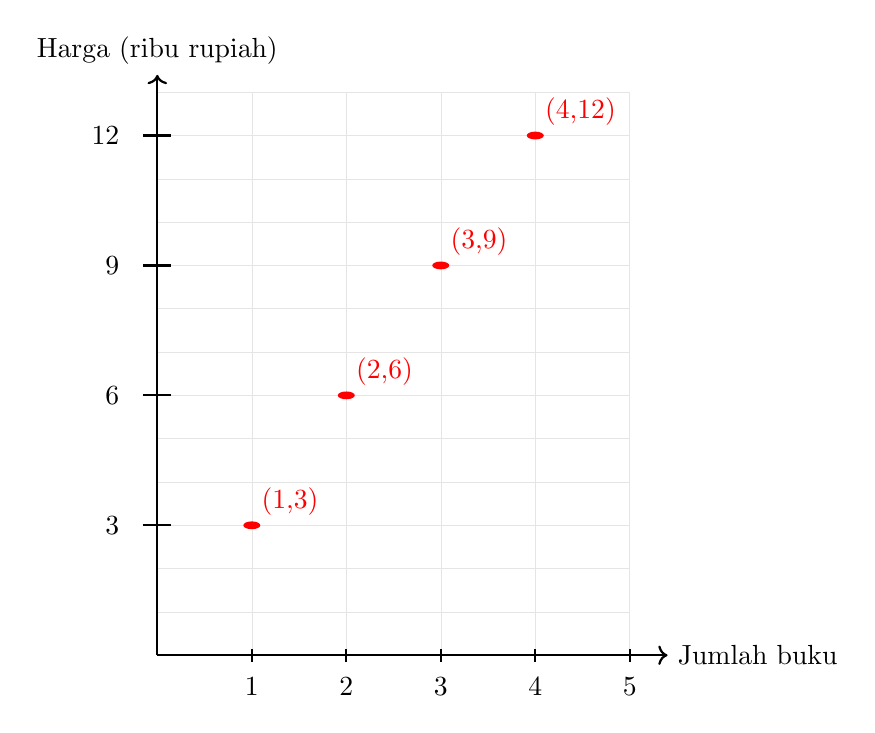
\begin{tikzpicture}[x=1.2cm, y=0.55cm]
  % Kisi-kisi tipis sebagai latar
  \draw[step=1, gray!20, very thin] (0,0) grid (5,13);
  % Sumbu mendatar: jumlah buku
  \draw[thick,->] (0,0) -- (5.4,0) node[right] {Jumlah buku};
  % Sumbu tegak: harga dalam ribuan rupiah
  \draw[thick,->] (0,0) -- (0,13.4) node[above] {Harga (ribu rupiah)};
  % Tanda pada sumbu mendatar
  \foreach \x in {1,...,5} {
    \draw[thick] (\x,-0.15) -- (\x,0.15);
    \node[below] at (\x,-0.3) {\x};
  }
  % Tanda pada sumbu tegak, setiap 3 ribu
  \foreach \y in {3,6,9,12} {
    \draw[thick] (-0.15,\y) -- (0.15,\y);
    \node[left] at (-0.3,\y) {\y};
  }
  % Titik-titik dari tabel harga buku
  \foreach \x/\y in {1/3, 2/6, 3/9, 4/12} {
    \fill[red] (\x,\y) circle (0.09);
    \node[above right, red] at (\x,\y) {(\x,\y)};
  }
\end{tikzpicture}

\section*{Grafik Perbandingan Senilai: Garis Lurus dari Titik Asal}

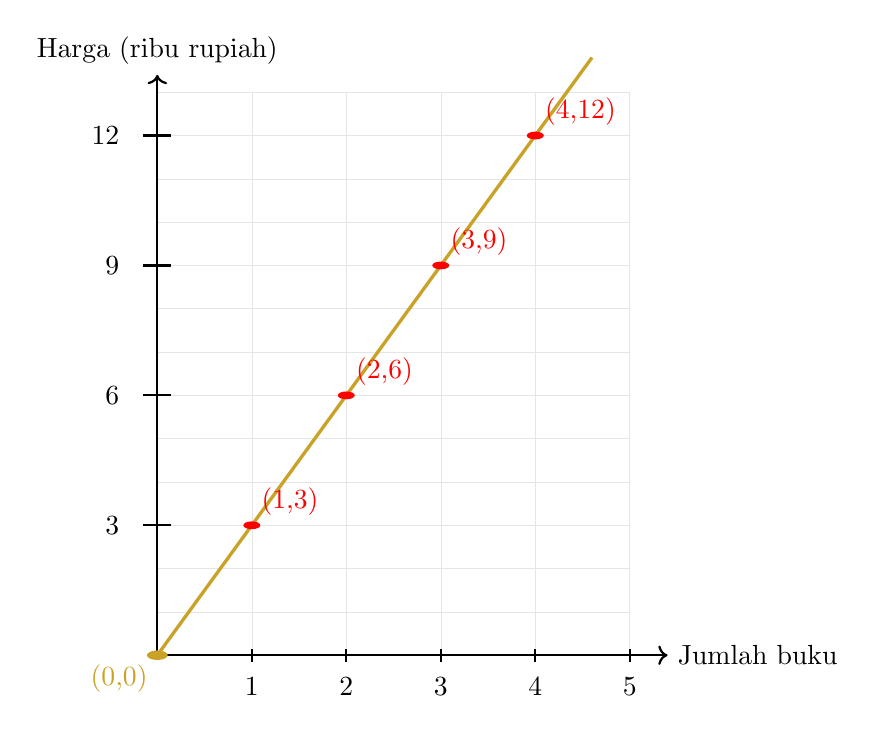
\begin{tikzpicture}[x=1.2cm, y=0.55cm]
  % Kisi-kisi tipis sebagai latar
  \draw[step=1, gray!20, very thin] (0,0) grid (5,13);
  % Sumbu mendatar: jumlah buku
  \draw[thick,->] (0,0) -- (5.4,0) node[right] {Jumlah buku};
  % Sumbu tegak: harga dalam ribuan rupiah
  \draw[thick,->] (0,0) -- (0,13.4) node[above] {Harga (ribu rupiah)};
  % Tanda pada sumbu mendatar
  \foreach \x in {1,...,5} {
    \draw[thick] (\x,-0.15) -- (\x,0.15);
    \node[below] at (\x,-0.3) {\x};
  }
  % Tanda pada sumbu tegak, setiap 3 ribu
  \foreach \y in {3,6,9,12} {
    \draw[thick] (-0.15,\y) -- (0.15,\y);
    \node[left] at (-0.3,\y) {\y};
  }
  % Garis perbandingan senilai: dari titik asal melewati semua titik
  \draw[very thick, color=goldenrod] (0,0) -- (4.6,13.8);
  % Titik-titik dari tabel harga buku
  \foreach \x/\y in {1/3, 2/6, 3/9, 4/12} {
    \fill[red] (\x,\y) circle (0.09);
    \node[above right, red] at (\x,\y) {(\x,\y)};
  }
  % Titik asal ditandai khusus
  \fill[goldenrod] (0,0) circle (0.11);
  \node[below left, color=goldenrod] at (0,0) {(0,0)};
\end{tikzpicture}

\end{document}
